\section{The RRT algorithm}
\label{sec:rrt-algorithm-intro}

The \ac{RRT} algorithm~\cite[LaValle]{article} is a tree based algorithm which,
starting at the intial configuration of the system, grows it's branches into the
unexplored parts of the state space through some suitable choice of distance
metric and sampling distribution for the problem at hand. The expansion is
divided up into three general steps, whereas the first is randomly, through some
probability distribution, choosing a configuration from the state space for
which the algorithm will try and expand towards. Secondly the algorithm finds
the node in the tree which is closest to the sample in the sense of some chosen
distance metric. Thirdly, it tries to connect the sample with the nearest node
in the tree through some predetermined expansion operator. If a connection can
be made -- meaning that it is collision free, and satisfies the constraints of
the dynamic model -- then a new node is added to the tree, and a vertice is made
between the two states. If the sampling distribution is uniform, then the tree
is known to have the attribute that the probability of expanding from an
existing node in the tree is proportional the the \textit{Voronoi region} of
that node, and as the largest Voronoi regions belong to the states on the leaves
of the tree. As the Voronoi regions divides a plane according to the
\textit{nearest neighbour rule}, each point is associated with the region of the
plane closest to
it~\cite{aurenhammerVoronoiDiagramsSurvey1991}~\cref{fig:voronoi-diagram}. This
means that the tree will quickly expand into unexplored parts of the state
space, as can be seen in~\cref{fig:rrt-expansion,fig:rrt-voronoi}~\cite{Lav06},
which is what makes the \ac{RRT} algorithm good at solving a wide variety of
planning problems, especially ones with a high dimensional state space.

\begin{figure}
  \centering \documentclass{standalone}
\usepackage[ruled]{algorithm2e}
\usepackage{mathtools}
\usepackage{amsmath}

\begin{document}

\begin{algorithm}[H]
  \caption{Simple RRT algorithm}

  \DontPrintSemicolon

  \KwIn{Initial configuration, \(q_{0}\)}
  \KwOut{\textit{RRT}-graph \(\mathcal{G}\)}

  \SetKwFunction{RandConf}{Sample\_Random\_Configuration}
  \SetKwFunction{NearestVertex}{Find\_Nearest\_Vertex}
  \SetKwFunction{NewConfig}{New\_Config}
  \SetKwFunction{AddVertex}{add\_vertex}
  \SetKwFunction{AddEdge}{add\_edge}

  \(\mathcal{G}.init(q_{0})\)
  \For{\(i \leftarrow 1\) \KwTo \(k\)}{
    \(q_{\textit{rand}} \leftarrow \) \RandConf{} \;
    \(q_{\textit{near}} \leftarrow \) \NearestVertex{\(q_{\textit{rand}}, \mathcal{G}\)}\;
    \(q_{\textit{new}} \leftarrow \) \NewConfig{\(q_{\textit{near}}, q_{\textit{rand}} \)}\;
    \(\mathcal{G}\).\AddVertex{\(q_{\textit{new}}\)}\;
    \(\mathcal{G}\).\AddEdge{\(q_{\textit{near}}, q_{\textit{new}}\)} \;
  }

\end{algorithm}

\end{document}
\end{figure}

\begin{figure}
  \centering
  \begin{minipage}[b]{0.3\textwidth}
    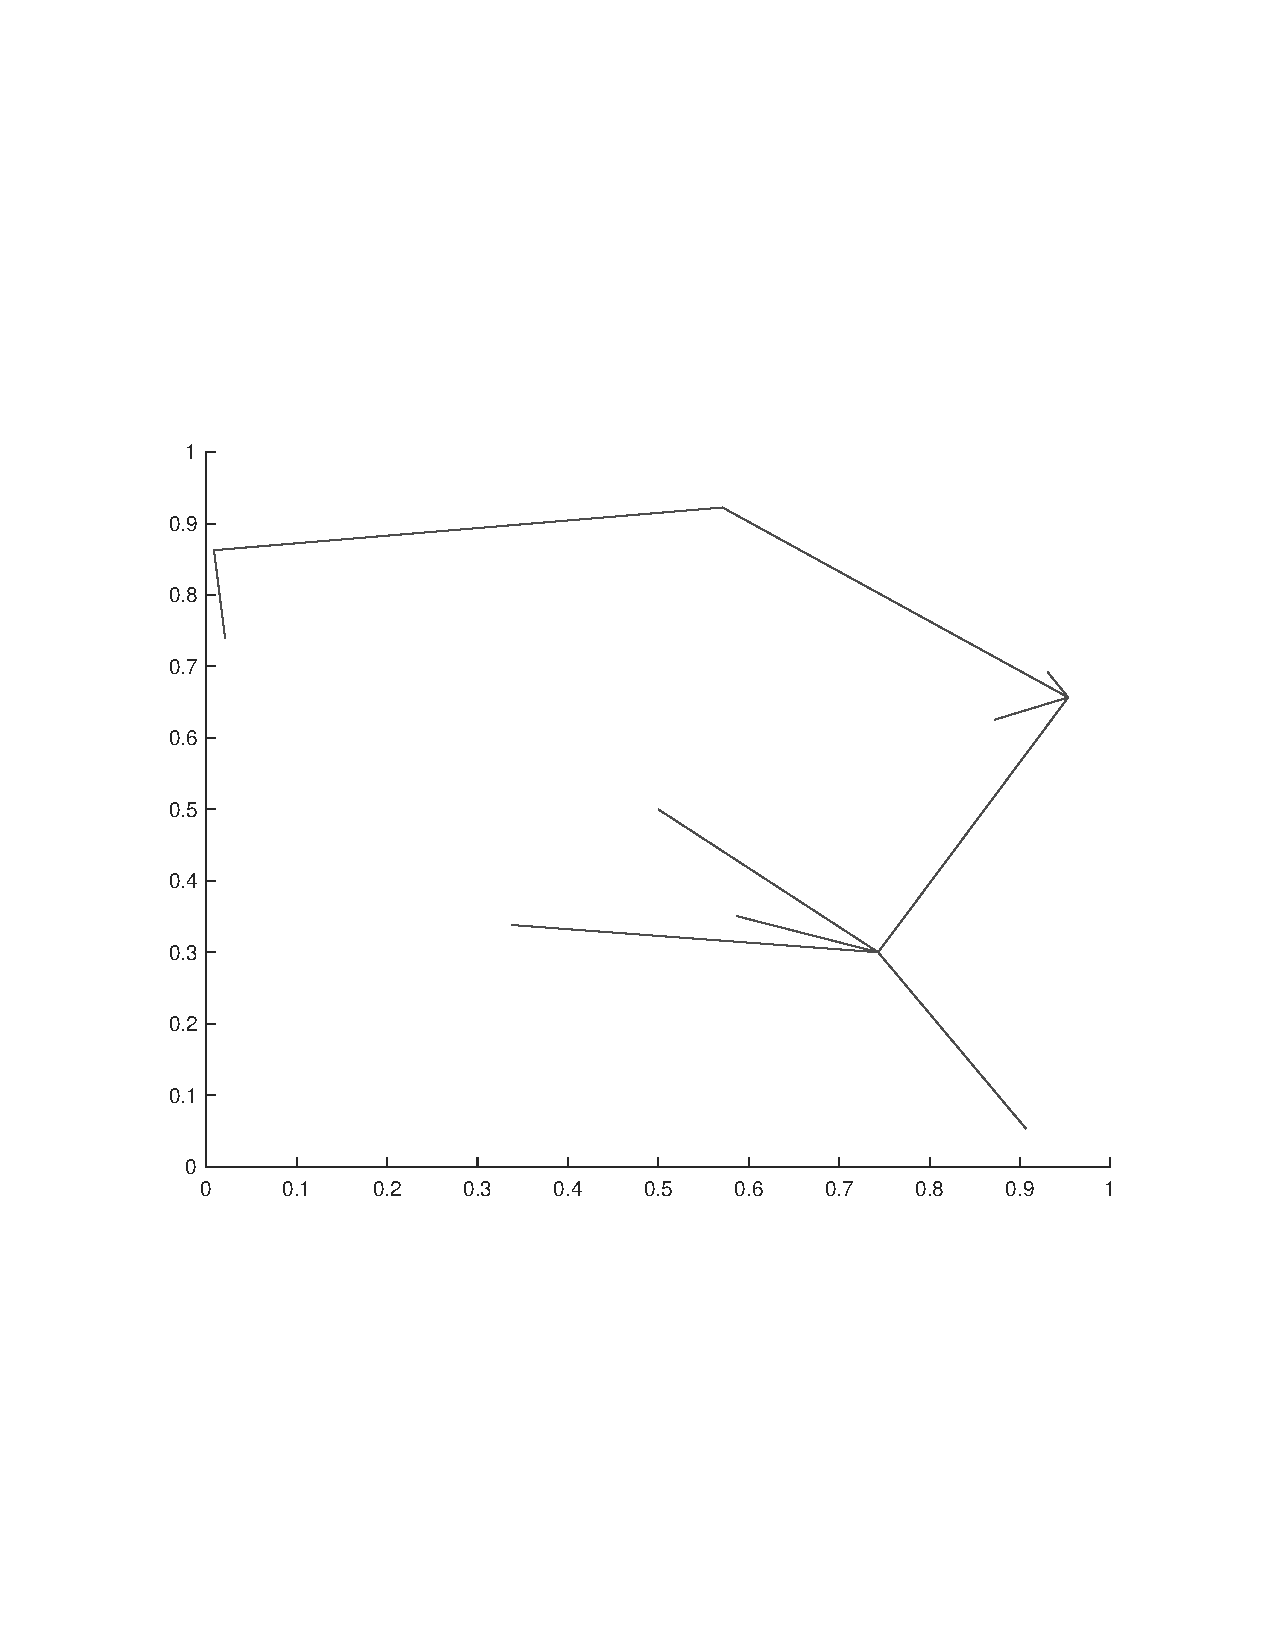
\includegraphics[width=\textwidth]{plainRRT10}
    \caption{RRT-tree after 10 iterations.}
  \end{minipage}
  \begin{minipage}[b]{0.3\textwidth}
    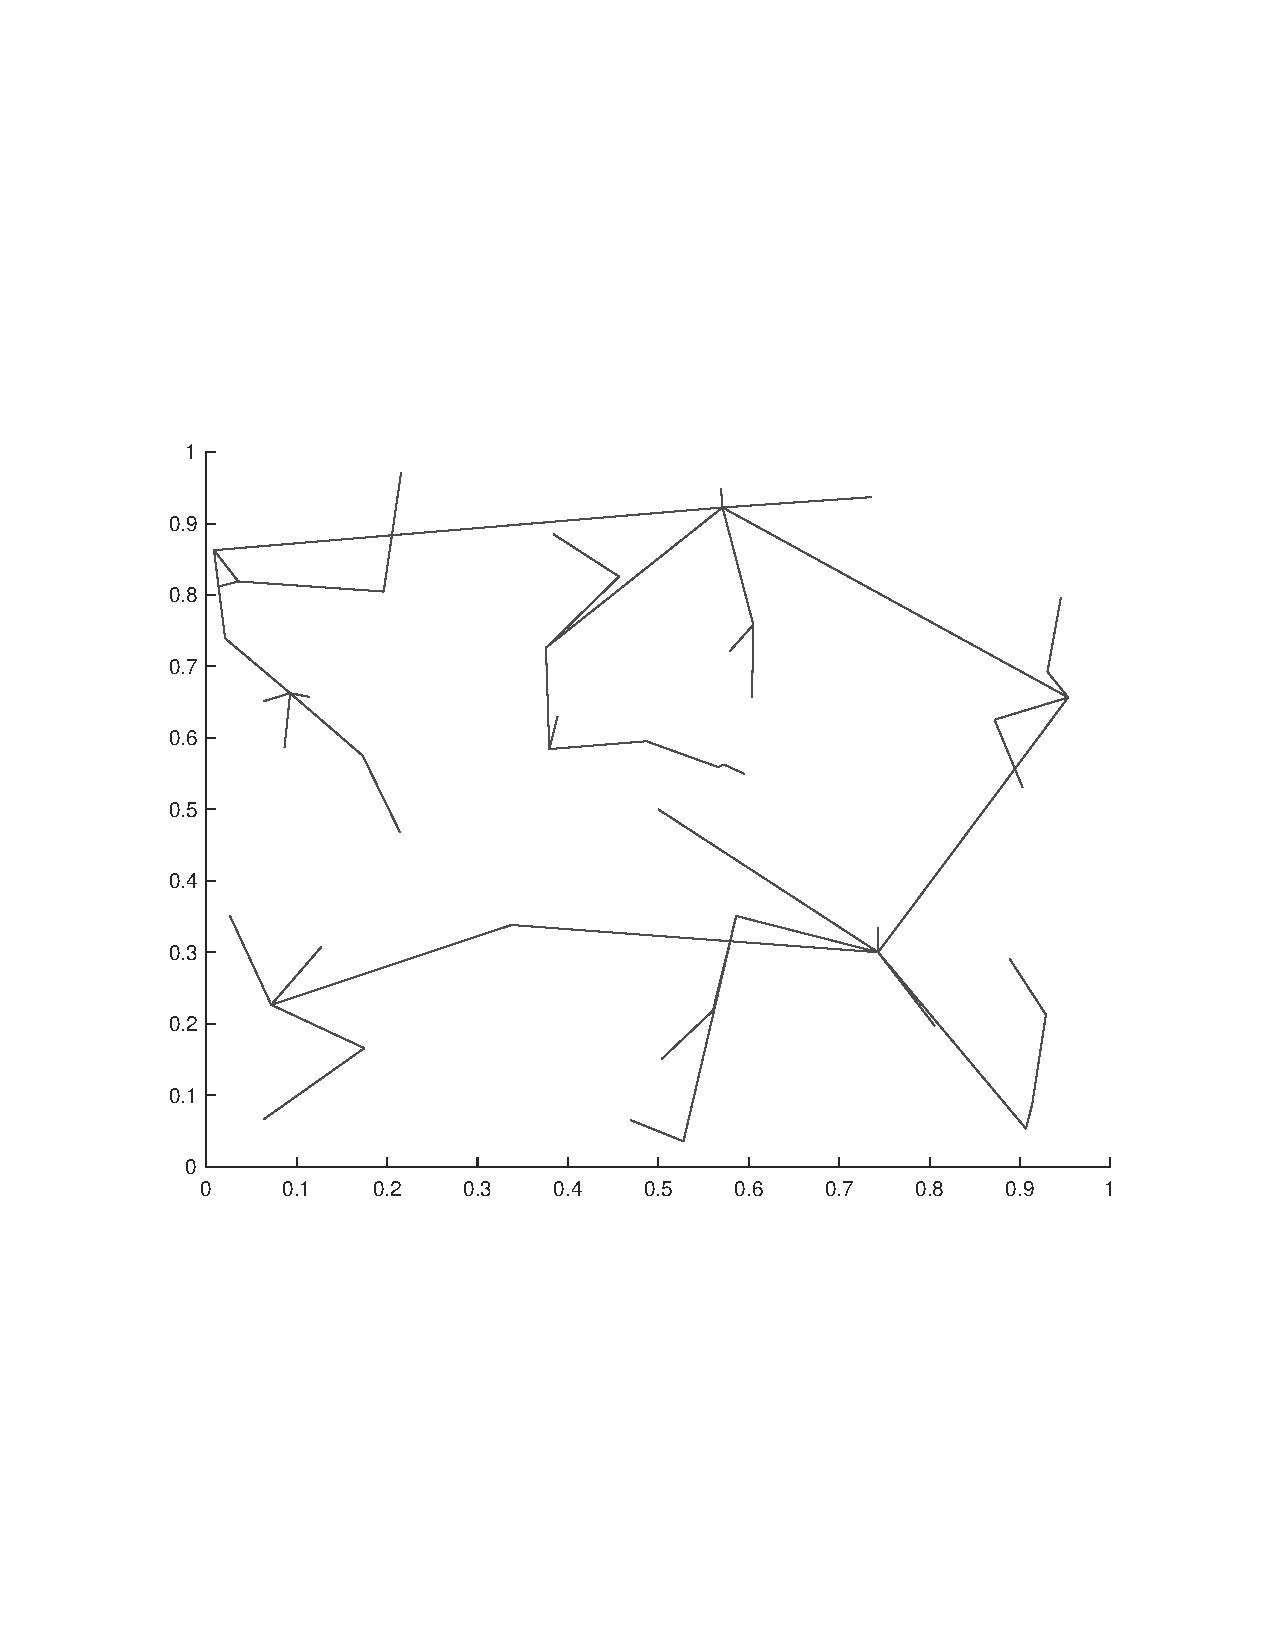
\includegraphics[width=\textwidth]{plainRRT50}
    \caption{RRT-tree after 50 iterations.}
  \end{minipage}
  \begin{minipage}[b]{0.3\textwidth}
    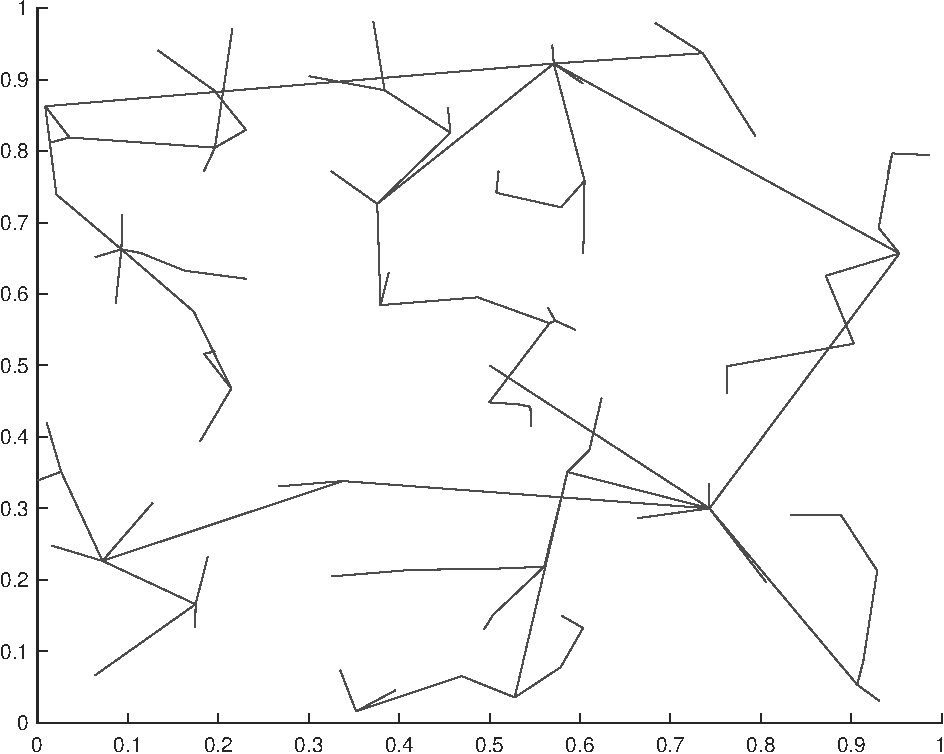
\includegraphics[width=\textwidth]{plainRRT100}
    \caption{RRT-tree after 100 iterations.}
  \end{minipage}
  \newline % Start the new line of plainRRT10.
  \begin{minipage}[b]{0.3\textwidth}
    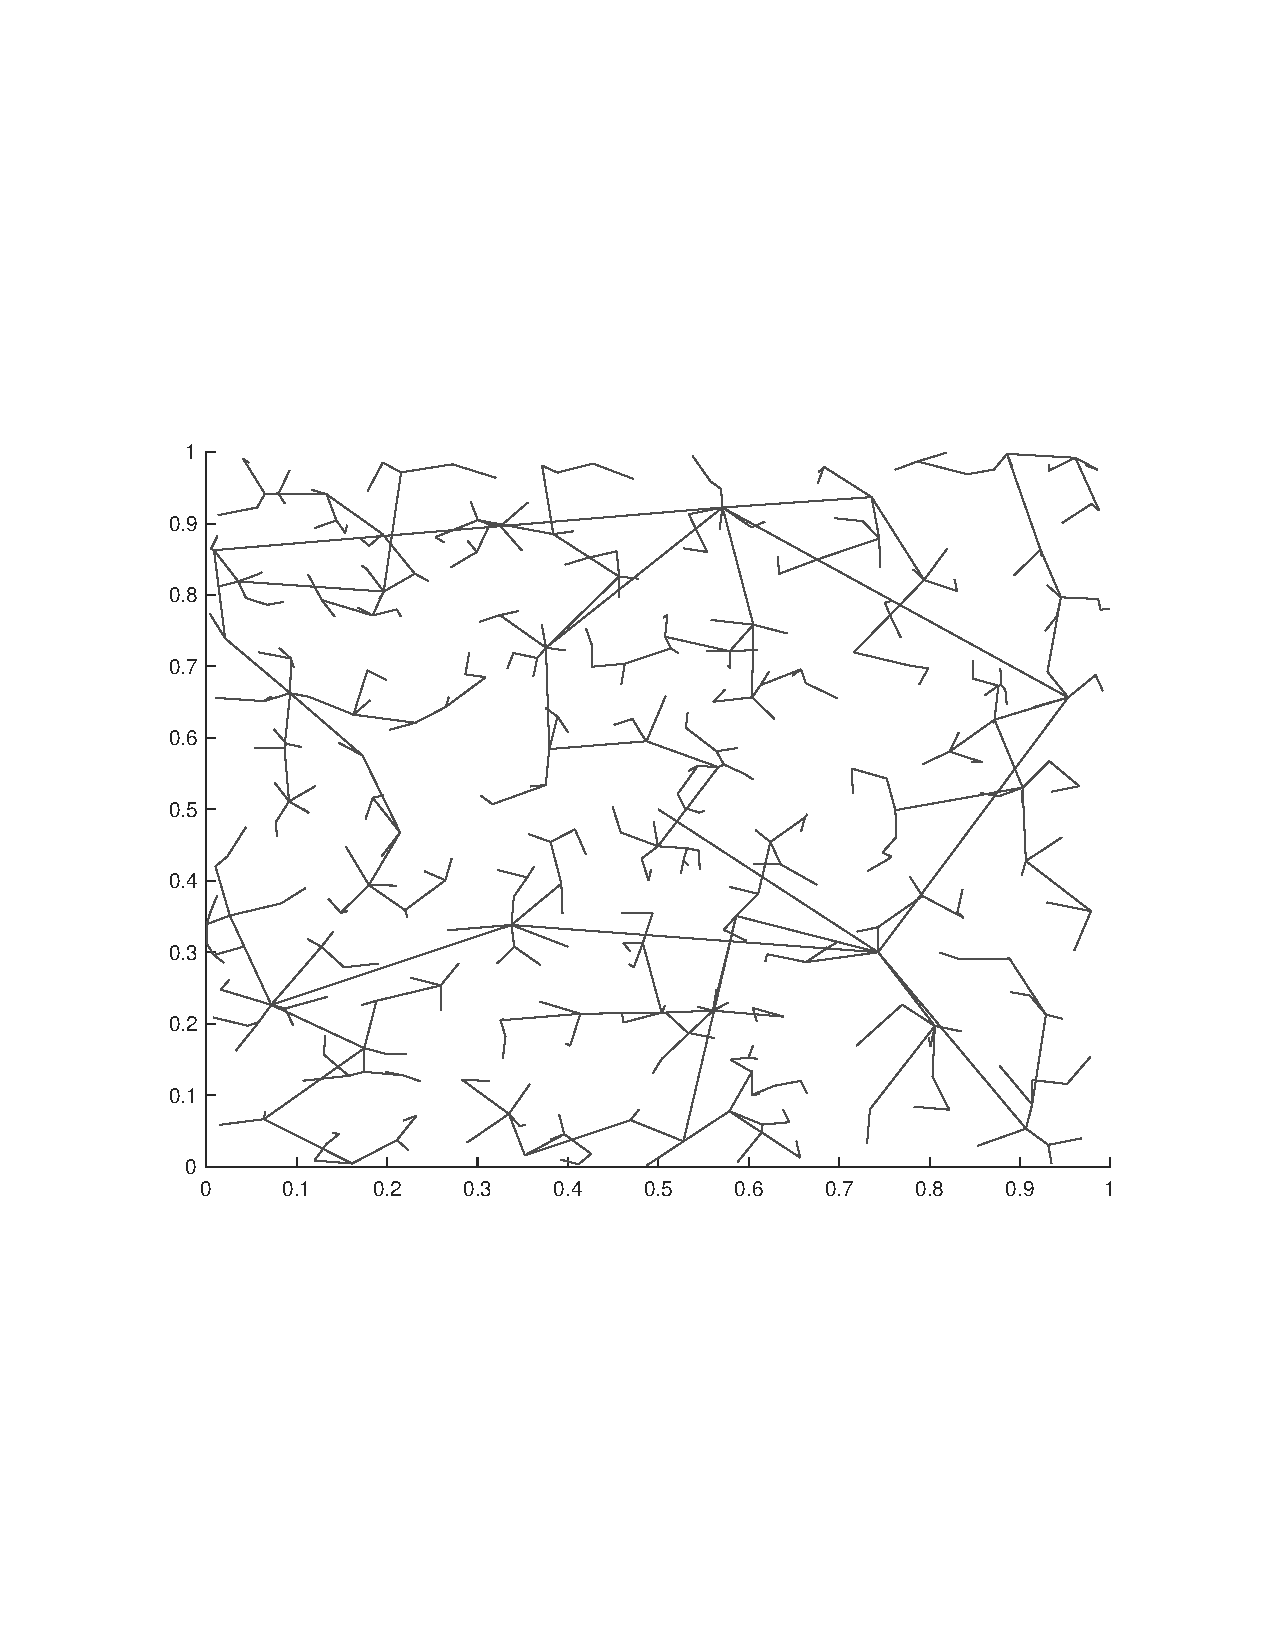
\includegraphics[width=\textwidth]{plainRRT500}
    \caption{RRT-tree after 500 iterations.}
  \end{minipage}
  \begin{minipage}[b]{0.3\textwidth}
    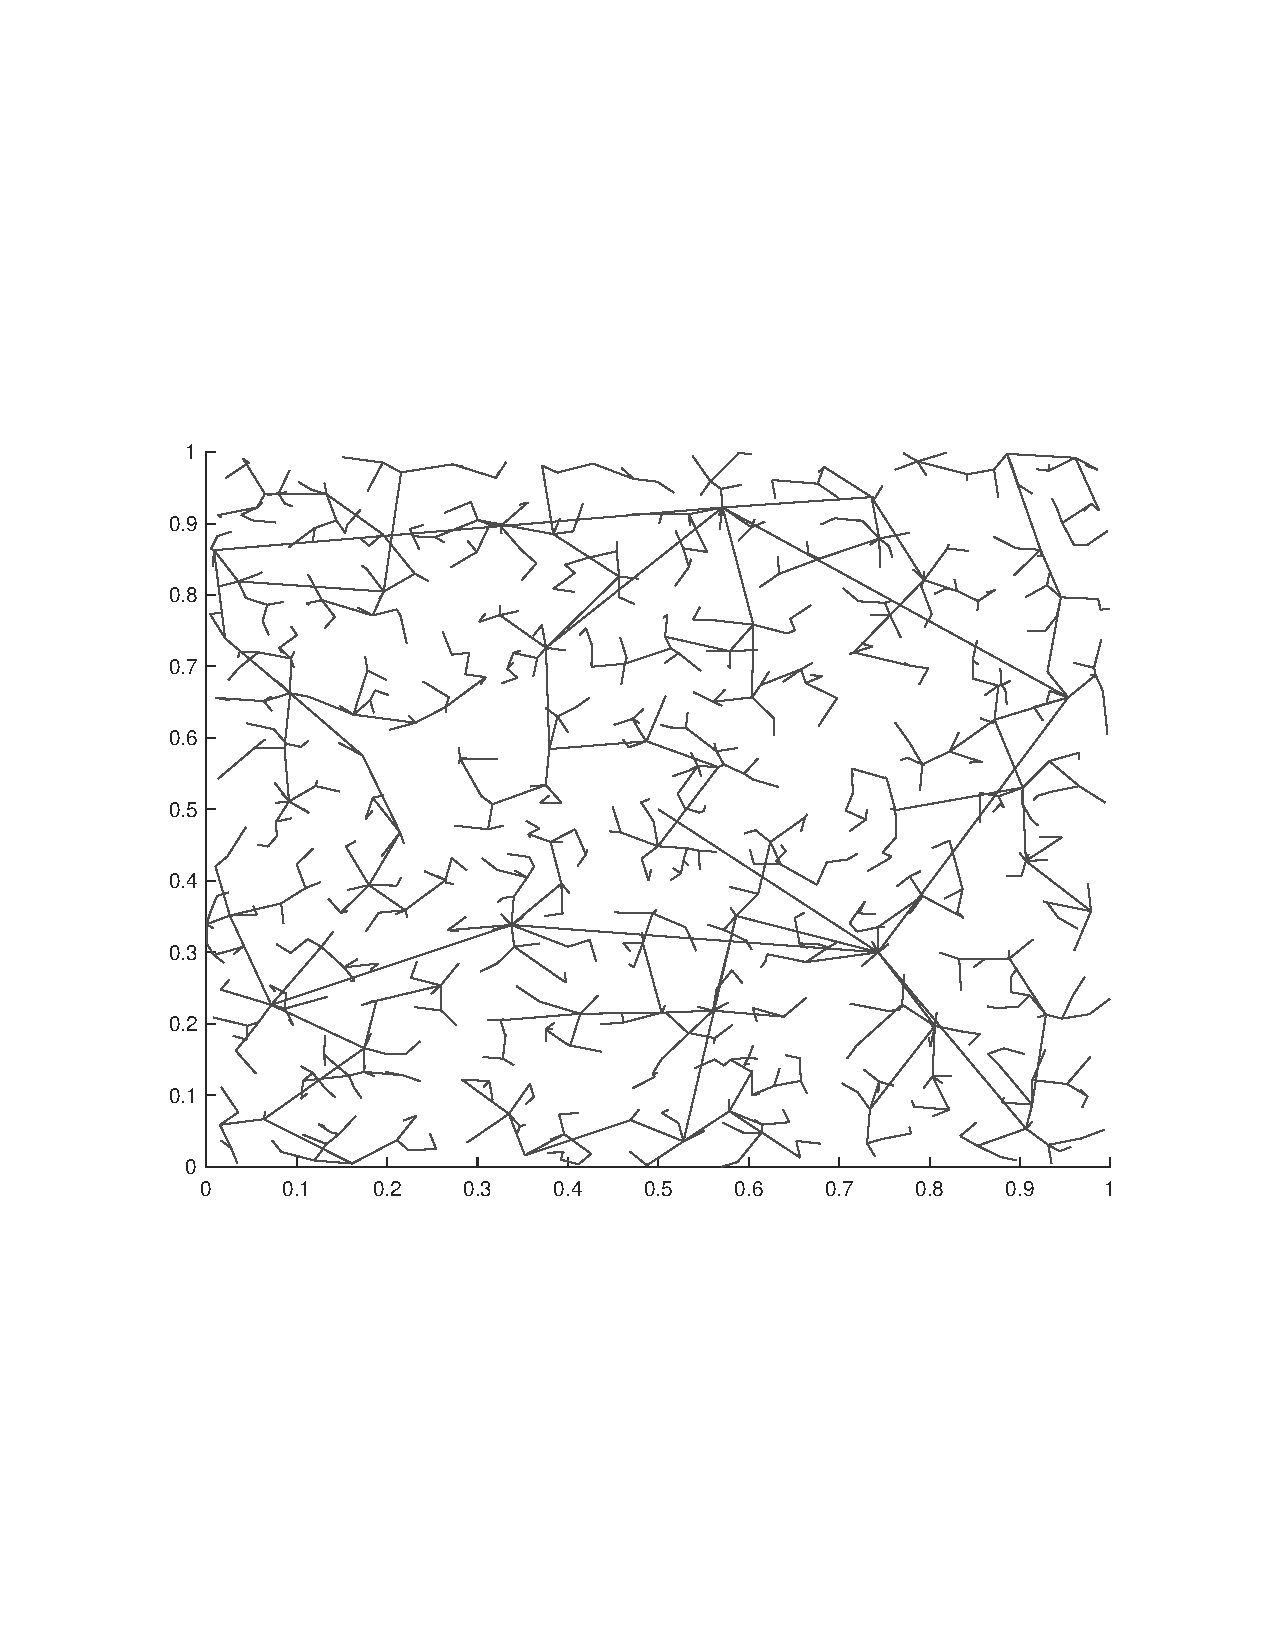
\includegraphics[width=\textwidth]{plainRRT1000}
    \caption{RRT-tree after 1000 iterations.}
  \end{minipage}
  \begin{minipage}[b]{0.3\textwidth}
    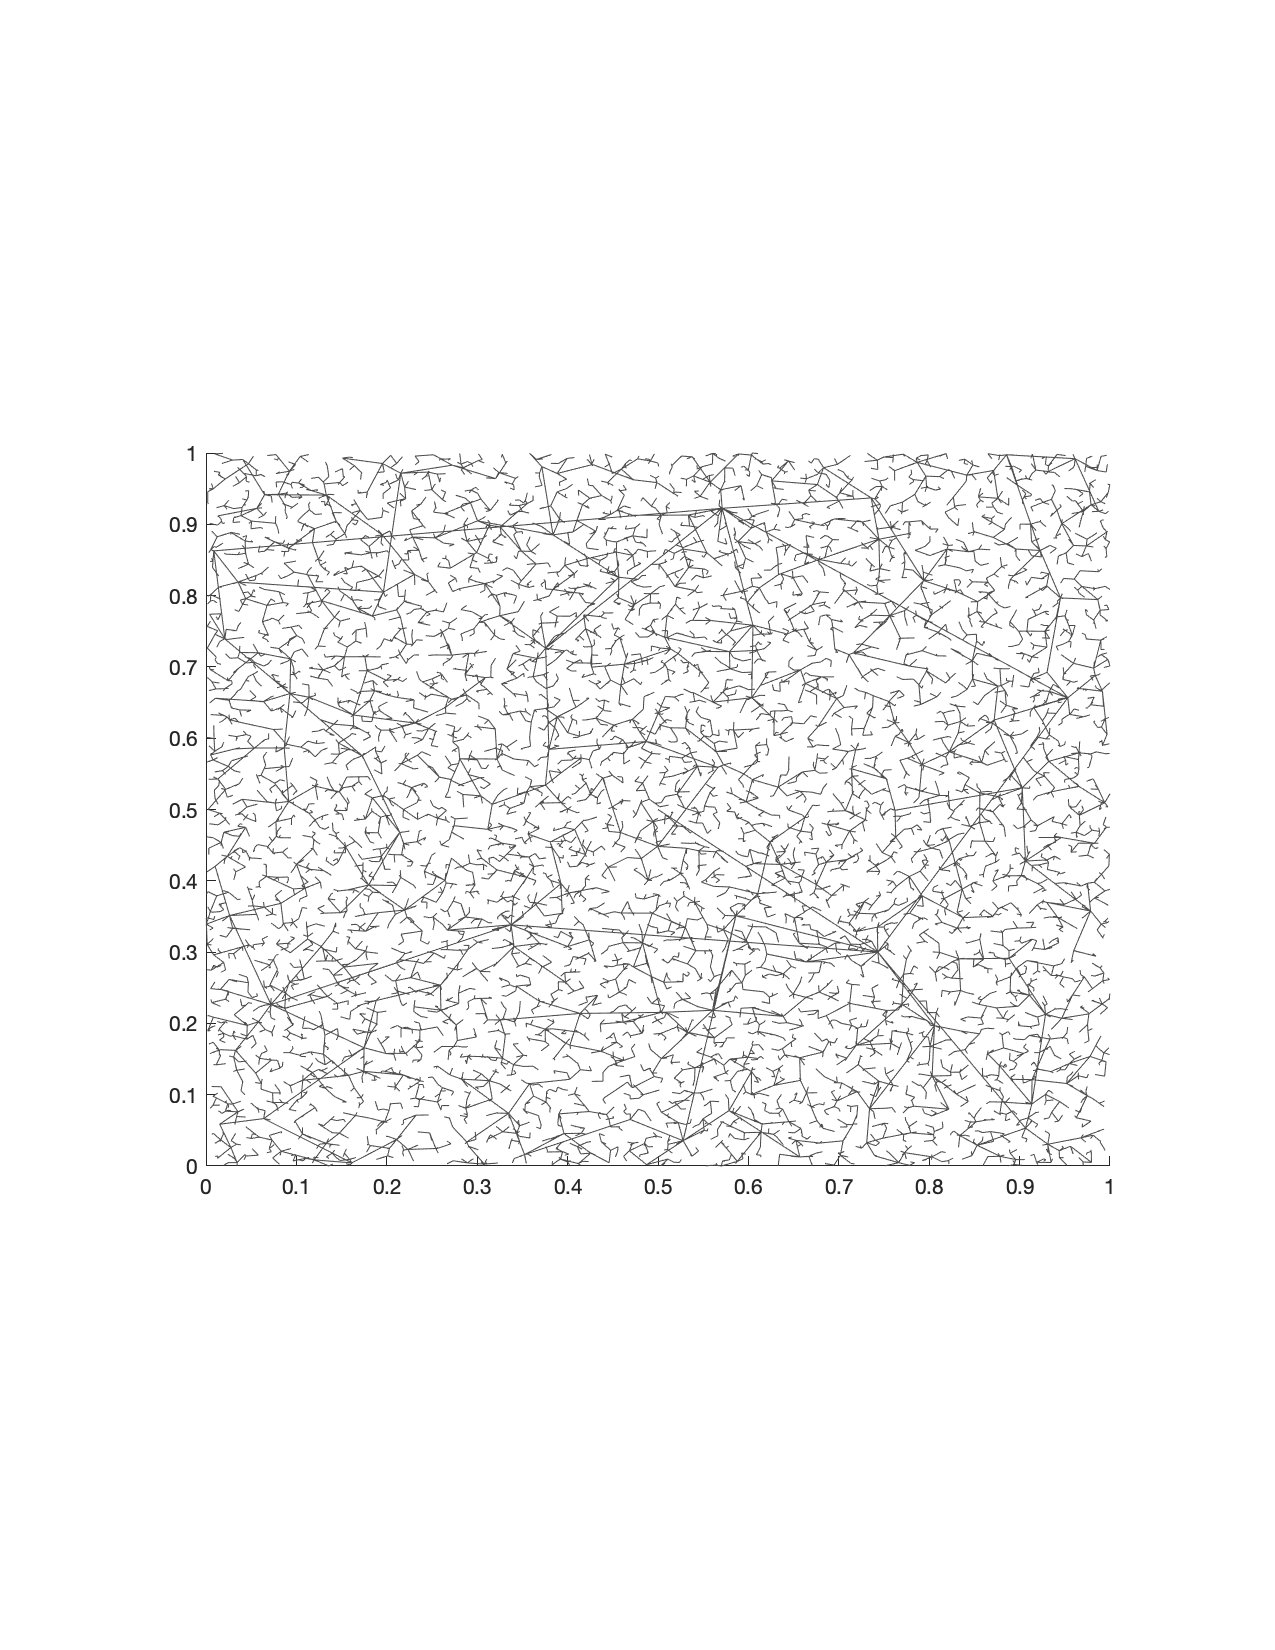
\includegraphics[width=\textwidth]{plainRRT10000}
    \caption{RRT-tree after 10000 iterations.}
  \end{minipage}
  \caption{Pictured: The \ac{RRT} algorithm quickly expanding deep into the
    state-space, then later, exploring the finer parts, until the exploration is
    complete.}
  \label{fig:rrt-expansion}
\end{figure}


\begin{figure}
  \centering 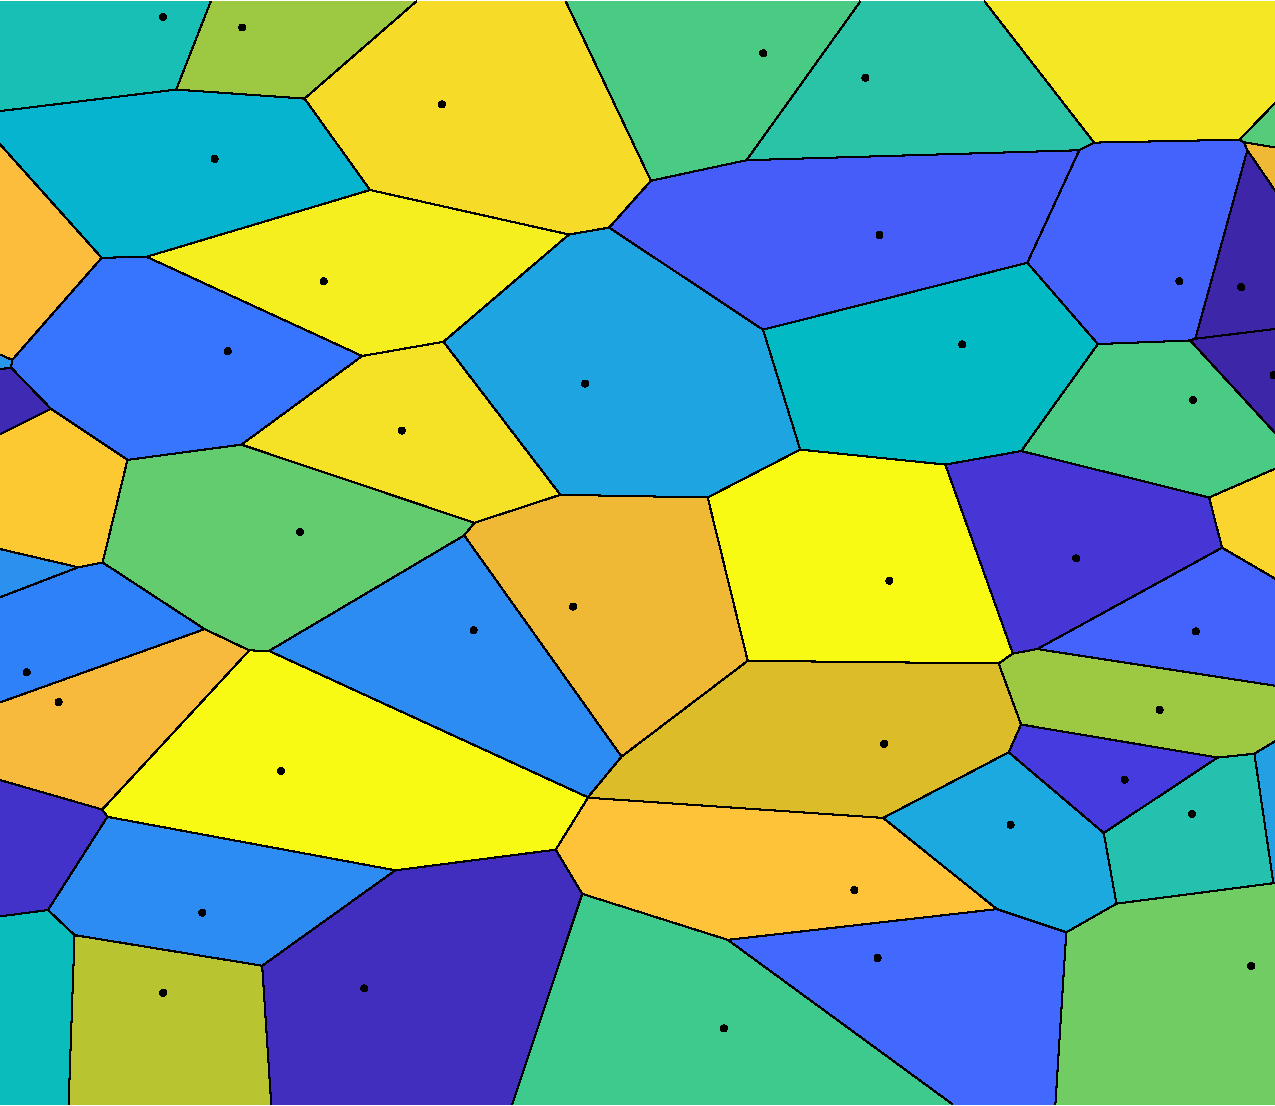
\includegraphics[scale=.3]{figures/rrt/voronoi-diagram}
  \caption{Pictured: The Voronoi regions for a collection of points in the
    plane, using the standard Euclidean metric.}
  \label{fig:voronoi-diagram}
\end{figure}

When inspecting the Voronoi regions of a \ac{RRT} tree, it is apparent that the
leaf nodes will have the largest Voronoi regions, and thus also the largest
probability for getting expanded, as can be seen in
figure~\cref{fig:rrt-voronoi}.

The \ac{RRT} algorithm is a discrete sampling based algorithm, noticeable for
its ability to handle large state-spaces. This stems from the algorithm's
ability to avoid the \textit{curse of dimensionality}, which means that it does
not suffer the same computational penalty with scaling the state space, as is
hampering a lot of motion planning algorithms~\cite{Lav06}. Still, even though
the \ac{RRT} algorithm is sampling based, it will, as time goes to infinity
achieve probabilistic completeness in the state-space. Which means that it will
cover the whole state space with the tree if given infinite time. Thus one can
expect the \ac{RRT} algorithm to find a solution, if one exists and the
algorithm is given enough time.

\begin{figure}
  \centering \frame{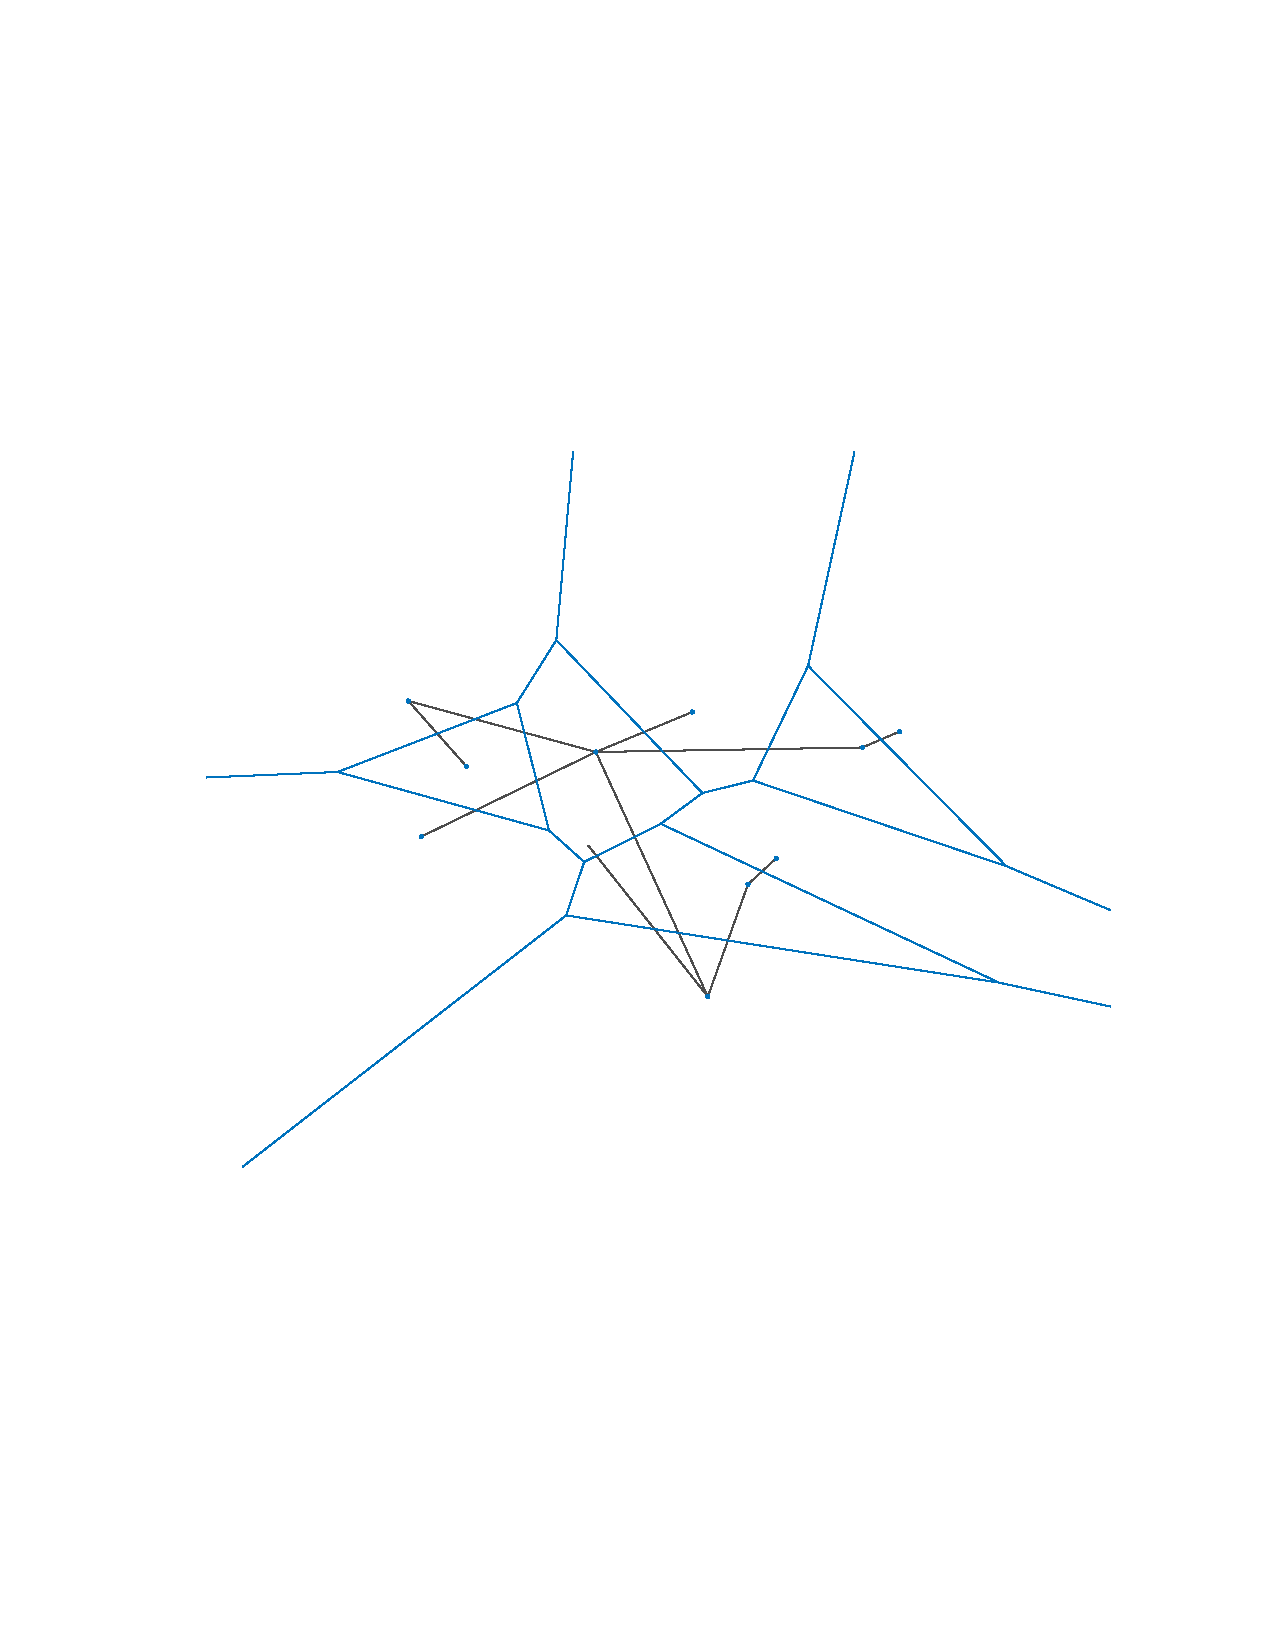
\includegraphics[clip, trim=5cm 9cm 5cm 9cm,
    scale=.5]{figures/rrt/rrtvoronoi}}
  \caption{Pictured: The voronoi regions for each node in a simple RRT tree,
    which shows how the voronoi bias will lead the algorithm towards unexplored
    areas quickly.}
  \label{fig:rrt-voronoi}
\end{figure}

\begin{figure}
  \documentclass{standalone}
\usepackage{tikz}

\begin{document}
    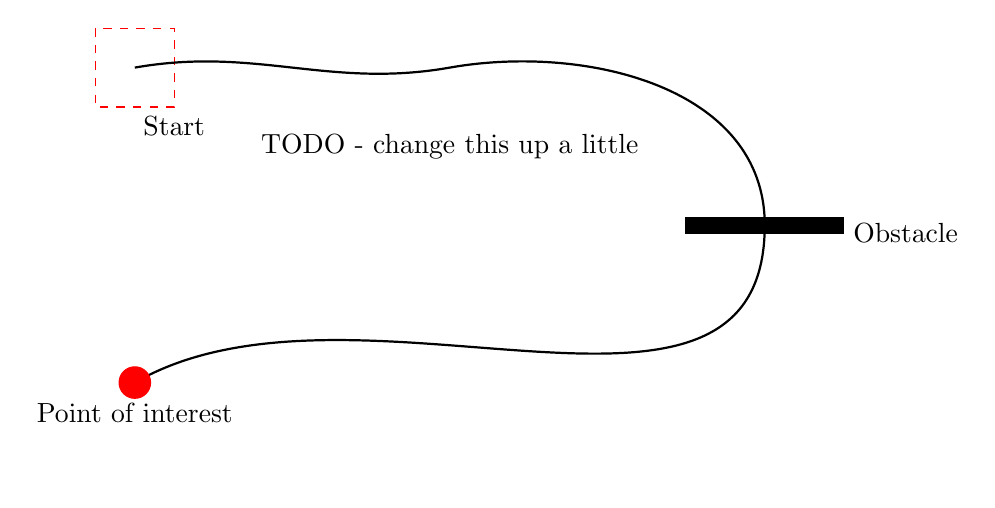
\begin{tikzpicture}
      \draw [red,dashed] (-2.5,2.5) rectangle (-1.5,1.5) node [black,below] {Start}; % Draws a rectangle
      \draw [thick] (-2,2) % Draws a line
      to [out=10,in=190] (2,2)
      to [out=10,in=90] (6,0) 
      to [out=-90,in=30] (-2,-2);    
      \draw [fill] (5,0.1) rectangle (7,-0.1) node [black,right] {Obstacle}; % Draws another rectangle
      \draw [red,fill] (-2,-2) circle [radius=0.2] node [black,below=4] {Point of interest}; % Draws a circle
      \draw node at (2,1) {TODO - change this up a little};
    \end{tikzpicture}
\end{document}
\end{figure}


\subsection{RRT's with motion primitives as extension operators}

There are multiple ways in which an \ac{RRT} algorithm can expand its planning
tree, with two main categories. One is where the extension, and the resulting
motions are calculated on the fly, and the other is where motions are computed
beforehand, and the planner chooses the most appropriate motion for which to
expand its tree. The \rrtfunnel{} algorithm falls into the latter category, and
as such the next section will build the basic theory for motion primitives in
motion planning.

\subsection{Motion Primitives}

The performance of the \ac{RRT} algorithm is dependent upon the control inputs
employed to search the state-space. For systems with few control inputs, random
control inputs can be sampled. The downside is that this usually produces
non-smooth motions. Instead, predefined motion primitives with known behaviour
can be sampled, which will produce a smoother path, while also reducing the
complexity of the planning task~\cite{vonasekGlobalMotionPlanning2013}, and if
shown on a humanoid robot in~\cite{hauserUsingMotionPrimitives2008}. A simple
basis of motion primitives for a vehicle can therefore be 'turn-left',
'go-straight', or 'turn-right'. By chaining these basic smooth motion primitves
together a smooth path from the intial- to the goal-state can be found. A figure
displaying a tree built up from the three motion primitives can be seen
in~\cref{fig:motion-primitive-tree}.

\begin{figure}
  \centering
  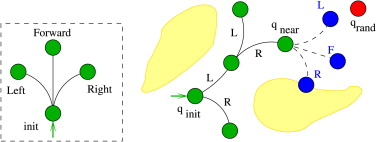
\includegraphics[scale=1]{figures/preliminaries/motion-primitive-tree}
  \caption{A simple motion primitive tree from the
    paper~\cite{vonasekHighlevelMotionPlanning2015}, displayinga a tree built
    from the composition of a left, right and a straight motion primitive.}
  \label{fig:motion-primitive-tree}
\end{figure}

Thus in essence robust motion primitives are beneficial as they seperate the
dynamics from the planner, enabling the planner to reason about what actions to
take, and not in what manner they should be executed. This observation is the
basis of the \rrtfunnel{}, which employs funnels as the robust motion primitives
and hence as the extension operators for the tree the planner employs, enabling
the \ac{RRT} part of the \rrtfunnel{} algorithm to remain oblivious to
uncertainties, and hence greatly simplifying the planning problem.

